\documentclass[../main.tex]{subfiles}

\begin{document}

 	\section{Illegale Drogenmärkte}
 	
 	\subsection{Definition}
 	
 	Illegale Drogenmärkte sind ein Bestandteil der Schattenwirtschaft und werden konkreter in die Kategorie der Schwarzmärkte eingeteilt.
 	Auf diesen Märkten werden hauptsächlich Substanzen gehandelt, die durch die regionale Drogenpolitik verboten oder reguliert werden.
 	Vor allem bekannt sind diese Märkte für ihre Kriminalität, namentlich Gewalt und Korruption.
 	Auch wenn die Anbieter und Nachfrager durch den Staat stark eingeschränkt werden, funktioniert der Markt nach den Grundprinzipien der Ökonomie.
 		
	
	\subsection{Marktteilnehmer}	
	
	\subsubsection{Anbieter}	
	Ein Anbieter im Schwarzmarkt nimmt generell immer eine höhere Position als der Nachfrager ein.
	Sie können wie Kartelle oder teilweise wie Monopole handeln und besitzen nahezu uneingeschränkte Macht über die Preisgestaltung.
	Händler können so hohe Margen anstreben und das potentielle Risiko durch einen Risikozuschlag ausgleichen.%
	\footnote{Vgl. \cite{becker-2006}.}
	Hohe Margen ziehen alle Arten von Händlern gleichermassen an.
	Neben der Preisgestaltung bringt auch das Fehlen der Justiz die Anbieter in eine höhere Position, da sie ohne Rechtsdurchsetzung ihre Forderungen mit Gewalt durchsetzen werden.%
	\footnote{Vgl. \cite{departmentofjustice-1994}.}
	Je höher man in der Lieferkette nach oben wandert, desto professioneller und gewalttätiger werden die Anbieter. 
	Dies führt dazu, dass man die Annahme tätigen kann, dass der Anbieter dem Nachfrager immer überlegen ist.\\
	
	\noindent
	Marketing gibt es kaum, da die Anbieter möglichst unauffällig agieren wollen.
	Die Kundenbindung erfolgt durch die Kunden, die mittels Mund-zu-Mund Propaganda den Anbietern neue Kunden liefern.
	Auf den ersten Blick existieren nur wenige Anreize für Innovation, da das nachgefragte Produkt in Theorie ziemlich heterogen ist und nur durch den Reinheitsgrad variieren kann.		
	Der grösste Teil der Innovation erfolgt nicht beim Produkt sondern bei den unternehmerischen Prozessen. 
	Eine Erhöhung der repressiven Massnahmen der Polizei kann zur Folge haben, dass Anbieter mehr in Sicherheit und Anonymität investieren.
	Die direkte Folge davon ist, dass der Handel immer professioneller und verdeckter wird.%
\footnote{Vgl. \cite{haucap-2018}.}
	Dieser Effekt wird im Kapitel \texttt{Illegale Drogenmärkte > Ökonomie > Preiselastizität} genauer analysiert.
	
	
	\subsubsection{Nachfrager}
	Die Interaktion zwischen Nachfrager und Anbieter basiert hauptsächlich auf Vertrauen.
	Gesetze können nicht auf das Handeln auf dem Markt angewendet werden, da beide Parteien illegal handeln und keine Partei eine Strafverfolgung riskieren will.
	Für Nachfrager existiert keine Sicherheit auf Qualität, Quantität und Verfügbarkeit der Güter.
	Sie können Opfer von Betrug aber auch Gewalttaten werden, ohne dass sie sich wehren können.%
	\footnote{Vgl. \cite{departmentofjustice-1994}.}\\
	
	\noindent	
	Die Endkonsumenten, ein Teil der Nachfrager, werden noch stärker als Händler, die als Nachfrager agieren, benachteiligt.
	Da Cannabis auch zu den suchterzeugenen Substanzen gezählt werden kann, werden die Prävalenzen der Konsumenten immer weiter steigen.%
	\footnote{Vgl. \cite{becker}.}
	Dies hat zur Folge, dass die Ausgaben der Konsumenten immer weiter steigen, bis sie nicht mehr in der Lage ihren Konsum zu finanzieren.
	Vielen Menschen bleiben in so einer Situation andere Möglichkeiten mehr übrig, so dass sie in die Beschaffungskriminalität abrutschen.%
	\footnote{Vgl. \cite{departmentofjustice-1994}.}
	
	
	\subsubsection{Staat}
	Der Staat nimmt eine passive Position im Markt ein und ist kein direkter Marktteilnehmer, versucht aber mit Gegenmassnahmen entgegenzuwirken.
	Während früher das einzige Mittel die vollständige Marktregulierung durch Repression war, werden heute nicht nur repressive Massnahmen getätigt.
	Die Viersäulenpolitik ist das wichtigste Mittel der Schweizer Drogenpolitk.
	Diese Politik ist seit der Revision des Betäubungsmittelgesetzes in \texttt{Art. 1a BetmG} ein fester Bestandteil der Drogenpolitik.
	\textit{(Siehe Abbildung \ref{fig:stgb-art-1a})}
	
	\begin{figure}[H]
	\begin{tcolorbox}
		\small
	 	\textbf{Art. 1a StGB - Vier-Säulen-Prinzip}\\[7pt]
	 	1. \quad Bund und Kantone sehen in folgenden vier Bereichen Massnahmen vor (Vier-Säulen-Prinzip):
		\begin{enumerate}[label=\alph*.]
			\item Prävention
			\item Therapie und Wiedereingliederung
			\item Schadenminderung und Überlebenshilfe
			\item Kontrolle und Repression
		\end{enumerate}
		2. \quad Bund und Kantone berücksichtigen dabei die Anliegen des allgemeinen Gesundheits- und Jugendschutzes
	\end{tcolorbox}	
	\captionsetup{font=small, skip=0pt}
	\caption{Rechtslage der Viersäulenpolitik}
	\label{fig:stgb-art-1a}
	\end{figure}
	 
  	\noindent
	In vier verschiedenen Bereichen werden Massnahmen getätigt, so dass das Schadensausmass des Drogenkonsums und Drogenhandels möglichst gering gehalten wird.
	Während die Repression beim Angebot ansetzt, versuchen die anderen Felder die Nachfrage senken.
	Beide Angehensweisen senken die Menge, jedoch verändert sich der Preis unterschiedlich. 
	Dieser Effekt wird im Kapitel der Preiselastizität genauer analysiert.\\
	
	\noindent
	Das seit 2016 bewährte Vier-Säulen-Modell wurde mit vier weiteren Handlungsfeldern erweitert. 
	Die Strategie wird vom Bundesamt für Gesundheit (BAG) festgelegt und in einem Bericht der Öffentlichkeit mitgeteilt.
	Neben den vier Hauptaufgaben wurden vier weitere Querschnittsaufgaben hinzugefügt.
	Die vier zusätzlichen Handlungsfelder dienen zur Steuerung und Koordination.
	Das Feld \textit{Koordination und Kooperation} dient dazu, bestehende Organisationen zu vernetzen und ihre Aktivitäten zu koordinieren.
	Das Feld \textit{Wissen} hat zum Ziel, neue Erkenntnisse zu Sucht zu generieren und zu vermitteln.
	Mit \textit{Sensibilisierung und Information} will der Bund die Gesellschaft über Sucht und Suchtprävention informieren, so dass sie sich im Ernstfall schützen können.
	Die \textit{Internationale Politik} zielt darauf ab, möglichst international vernetzt zu sein, um die grösstmögliche Datenbasis zur Verfügung zu haben.%
	\footnote{Vgl. \cite{bag-01}.}
	\textit{(Siehe Abbildung \ref{fig:vsp})}

	\noindent	 
	\begin{figure}[H]
		\centering
		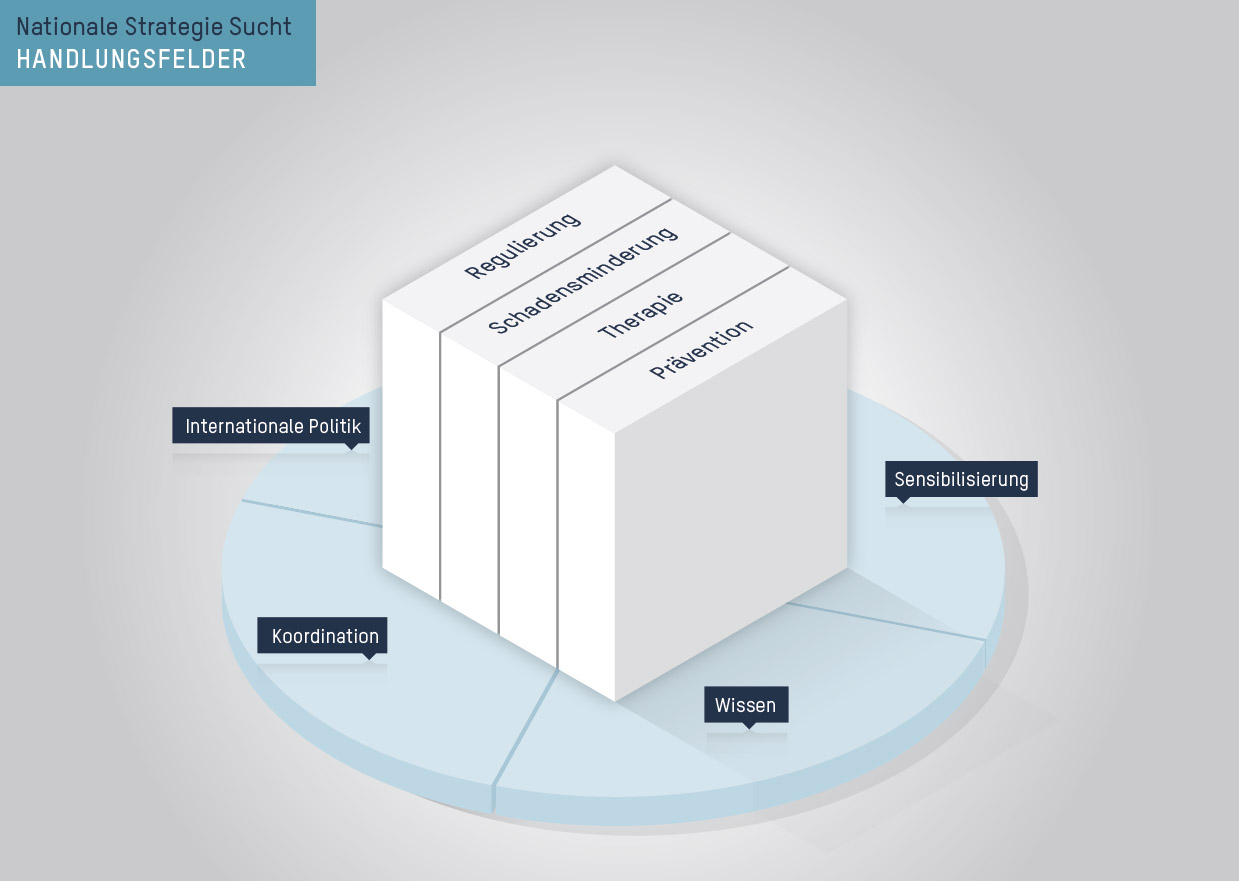
\includegraphics[width=0.8\linewidth]{VSP-erweitert}
		\captionsetup{font=small}
		\caption[Erweiterung der Viersäulenpolitik]{Erweiterung der Viersäulenpolitik\protect\footnotemark}		
		\label{fig:vsp}
	\end{figure}
	\footnotetext{\cite{bag-01}.}
	
	\subsection{Sozioökonomie}
	
	\paragraph{Datenbasis}
	Als Datenbasis dient eine Umfrage vom Suchtmonitoring Schweiz.%
	\footnote{Vgl. \cite{gmel}.}
	Die Prävalenz gibt an, wie viele Konsumenten in einem gewissen Zeitbereich Cannabis konsumiert haben.
	Die Lebenszeitprävalenz stellt dar, wie viele Schweizer mindestens einmal in ihrem Leben Cannabis konsumiert haben.
	Diese Regel gilt nach gleichem Prinzip für die 12-Monatsprävalenz und die 30-Tagesprävalenz.
	
	\paragraph{Prävalenz}	
	Gemäss einer Befragung des Suchtmonitoring haben 33.8\% der Schweizer Bevölkerung schon einmal in ihrem Leben Cannabis konsumiert.
	Die Tendenz ist seit Jahren leicht steigend und scheint auch kein Ende zu nehmen. 
	So stieg die Lebenszeitprävalenz in 5 Jahren (2011 bis 2016) um 5 Prozentpunkte. 
	Der Konsum ist in allen Altersklassen präsent und es herrscht keine generelle Abneigung gegenüber dem Konsum. 
	\textit{(Siehe Abbildung \ref{fig:langzeitpravalenz})}
	Es zeichnet sich klar ab, dass vor allem jüngere Leute Cannabis konsumieren. 
	Bei der jüngeren Bevölkerung von 20-34 Jahren ist es sogar die Mehrheit, die mindestens einmal in ihrem Leben Cannabis konsumiert hat.	
	
	\noindent	 
	\begin{figure}[H]
		\raggedleft
		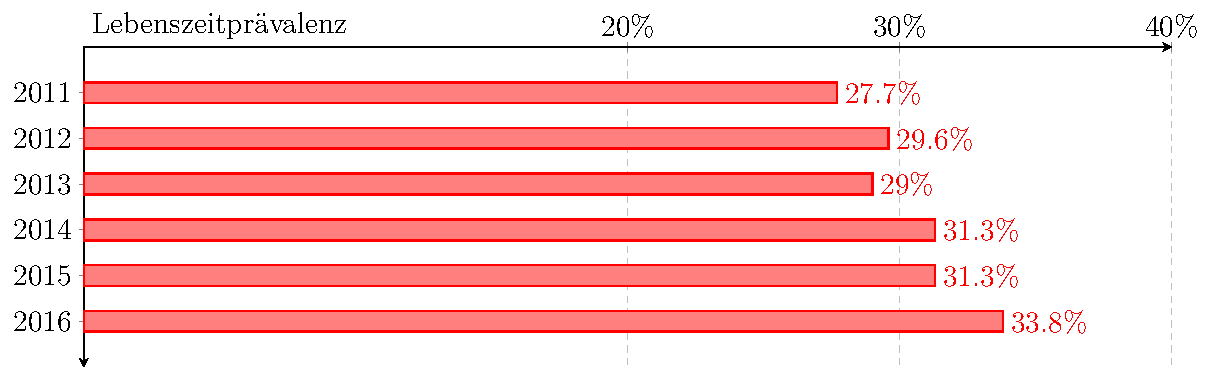
\includegraphics[height=4.56cm]{../figures/druguse-longtime}
		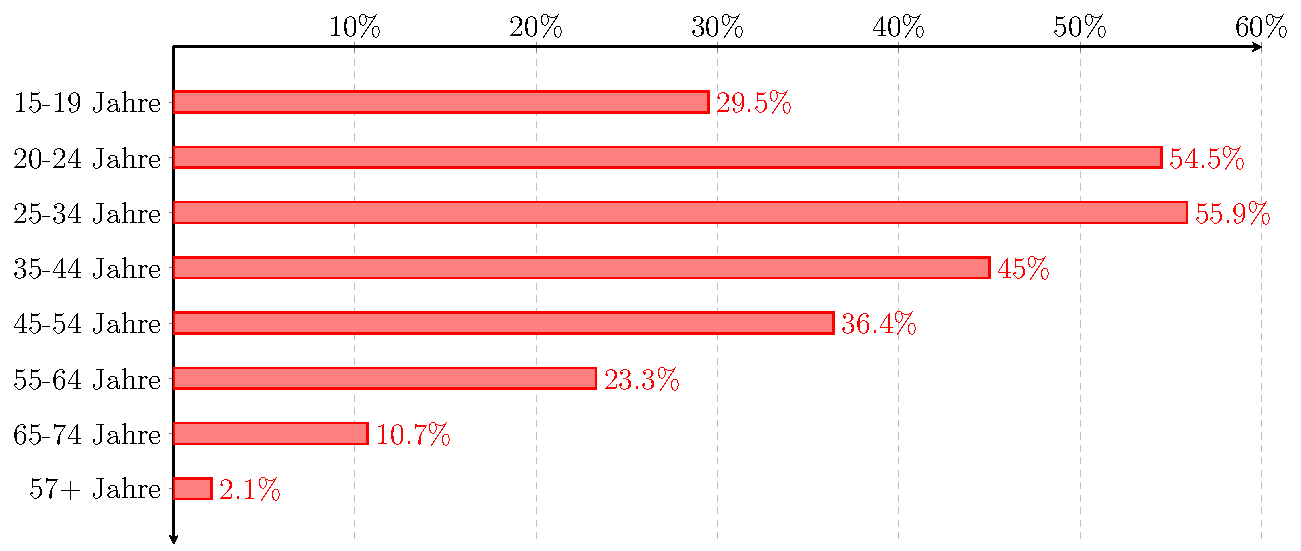
\includegraphics[height=6.71cm]{../figures/druguse-longtime-age}
		\captionsetup{font=small}
		\caption[Lebenszeitprävalenz von Cannabis]{Lebenszeitprävalenz von Cannabis\protect\footnotemark}
		\label{fig:langzeitpravalenz}		
	\end{figure}%
	\footnotetext{Eigene Abbildung. Vgl. \cite[85]{gmel}.}
	
	
	\noindent
	Die 12-Monatsprävalenz ist von 5.0\% auf 7.3\% gestiegen, während die 30-Tagesprävalenz keinen grossen Anstieg aufzeigt. 
	Anhand dem Verhältnis der beiden Prävalenzen kann man erkennen, dass der chonische Konsum kaum angestiegen ist, jedoch die Bereitschaft zum Probekonsum gestiegen ist. 
	Man kann annehmen, dass der Probierkonsum weiterhin ansteigen wird und sich dies in Zukunft in der Lebenszeitprävalenz zeigen wird.
	Die Entwicklung verrät auch, dass die Gesellschaft den Konsum nicht mehr stigmatisiert, auch wenn sie nicht regelmässig konsumiert.
	\textit{(Siehe Abbildung \ref{fig:kurzzeitpravalenz})}
	
	\noindent	 
	\begin{figure}[H]
		\centering
		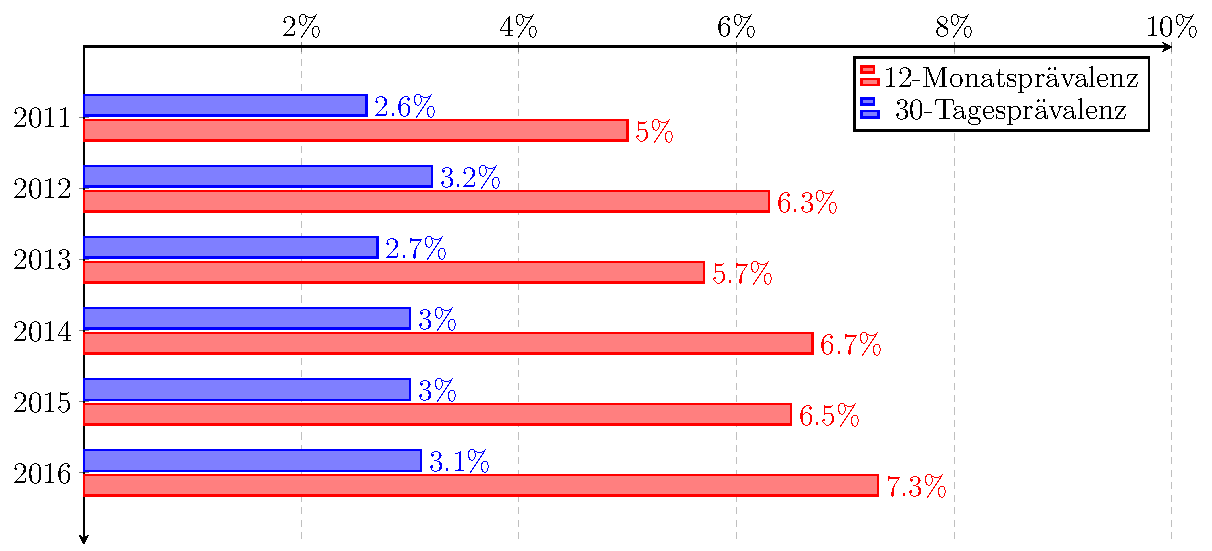
\includegraphics[height=6.5cm]{../figures/druguse-shorttime}
		\captionsetup{font=small}
		\caption[12-Monats- und 30-Tageprävalenz von Cannabis]{12-Monats- und 30-Tageprävalenz von Cannabis\protect\footnotemark}	
		\label{fig:kurzzeitpravalenz}	
	\end{figure}
	\footnotetext{Eigene Abbildung. Vgl. \cite[86]{gmel}.}
	
	\paragraph{Vergleich}
	Im Vergleich zu anderen illegalen Drogen hat Cannabis einen grossen Vorsprung.
	Die Lebenszeitprävalenz von den zwei nächsthöchten Substanzen sind wesentlich kleiner.
	Es konsumierten im Jahr 2016 4.2\% aller Schweizer mindestens einmal in ihrem Leben Kokain und 3.9\% Ecstasy.
	Der fast achtfache Unterschied lässt darauf schliessen, dass man Cannabis nicht gleich behandeln kann wie andere illegale Substanzen. 
	\textit{(Siehe Abbildung \ref{fig:otherdrugs})}
	
	\noindent
	\begin{figure}[H]
		\centering
		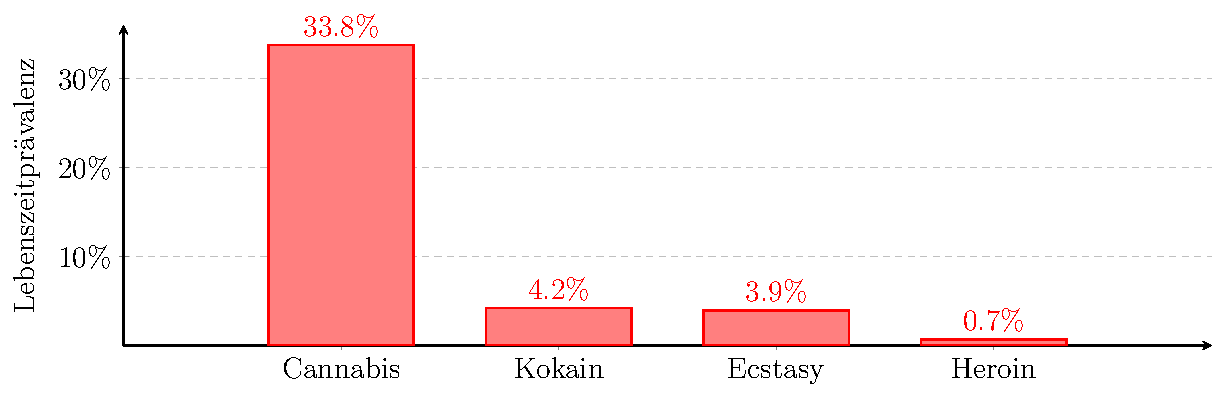
\includegraphics[height=5cm]{../figures/druguse-other}
		\captionsetup{font=small, skip=0pt}
		\caption[Prävalenzvergleich mit anderen Drogen]{Prävalenzvergleich mit anderen Drogen\protect\footnotemark}		
		\label{fig:otherdrugs}
	\end{figure}
	\footnotetext{Eigene Abbildung. Vgl. \cite[85-96]{gmel}.}
	
	\paragraph{Schlussfolgerung}
	Aus den Daten erkennt man, dass Cannabis einen anderen Stellenwert in der Gesellschaft hat wie andere illegale Drogen.
	Der Konsum ist mittlerweile weit verbreitet und wird auch von der Mehrheit akzeptiert.
	Dies ist eine Voraussetzung, dass man überhaupt eine Legalisierung in Betracht ziehen kann.
	Das Verbot scheint nicht die gewünschte Wirkung zu zeigen und die Entwicklung zeigt, dass immer weniger Schweizer das Gesetz beachten.
	Das Ziel der Prohibition ist es, den Konsum der Bevölkerung zu senken, jedoch steigen die Prävalenzen seit der Einführung der Prohibition.
	Da die repressiven Massnahmen nicht funktionieren, müsste man untersuchen, ob und wie man mit einer Legalisierung dennoch die kurzzeitigen Prävalenzen tief halten kann.
	
	
	\subsection{Ökonomie}
	
	\paragraph{Preis}
	Der durchschnittliche Preis für Cannabis befindet sich bei CHF 10.-, während der Preis von Haschisch mit CHF 13.- höher liegt.%
	\footnote{Vgl. \cite{zobel}.}
	Den erhöhten Preis von Haschisch kann man so erklären, dass die Wirkung meistens viel potenter ausfällt und die Herstellung aufwendiger ist.\\
	
	\noindent
	Der THC Gehalt von Haschisch übersteigt bei weitem den THC Gehalt von Cannabis.
	Der Preis wurde durch den Risikozuschlag und den hohen Margen in die Höhe getrieben.
	Der eigentliche Marktpreis von THC-haltigem Cannabis liegt weitaus tiefer und wird im Kapitel \texttt{Die marktwirtschaftliche Legalisierung} genauer ermittelt.
	
	\paragraph{Preiselastizität}
	Die Preiselastizität zeigt an, wie stark das Angebot oder die Nachfrage auf eine Preisänderung reagiert.
	Bei Cannabis wird die Preiselastizität der Nachfrage wie bei vielen Suchtmitteln sehr unelastisch eingeschätzt $(-1<\varepsilon_{xy}<0)$. 
	Nach einer Studie beträgt der Wert für die Preiselastizität der Nachfrage -0.54\%.%
	\footnote{Vgl. \cite{golzar}.}
	Die Preiselastizität von -0.54 ist der direkte Auslöser, dass eine Preiserhöhung von 1\% einen Nachfragerückgang von 0.54\% zur Folge hat.\\
	
	\noindent
	Eine Prohibition wirkt aufgrund der unelastischen Nachfragekurve nicht positiv ein.
	Eine Verschärfung der Strafverfolgung der Händler und Produzenten bewirkt keinen grossen Rückgang der Nachfrage, jedoch eine Erhöhung des Preises.
	Die Händler schlagen auf ihre Preise einen Risikozuschlag auf und wälzen diesen an ihre Kunden ab.
	Da die Konsumenten aufgrund ihrer Sucht jedoch nicht auf ihr Gut verzichten können, sinkt die Nachfrage kaum.
	\textit{(Siehe Abbildung \ref{fig:repression})}\\
	
	\noindent
	\begin{figure}[H]
		\centering
		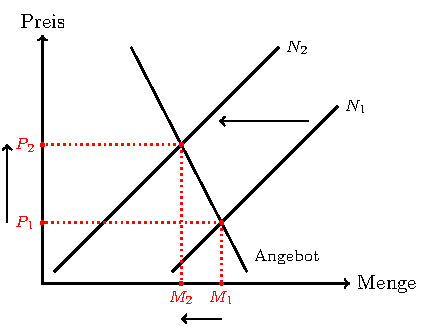
\includegraphics[height=9cm]{../figures/priceelasticity-repression}
		\captionsetup{font=small}
		\caption[Preiselastizität der Repression]{Preiselastizität der Repression\protect\footnotemark}		
		\label{fig:repression}
	\end{figure}
	\footnotetext{Eigene Abbildung.}
	
	\noindent
	Dieser Effekt wurde bereits analysiert und nennt man "rational addiction".
	Aus ökonomischer Sicht bringt die Prohibition nur bedingt einen Erfolg in der Bekämpfung des Drogenkonsums. 
	Auf den ersten Blick scheint sie die gewünschte Wirkung zu zeigen, jedoch entsteht dadurch ein anderer Nebeneffekt. 
	Dadurch dass die Preise steigen und die Nachfrage kaum zurückgehen kann, sind die Konsumenten gezwungen, die hohen Geldsummen zu bezahlen.
	Dies führt zu einer erhöhten Beschaffungskriminalität in der unteren Gesellschaftsschicht, somit ergibt sich eine erhöhte Kriminalität. %
	\footnote{Vgl. \cite{becker}.}
	Eine erhöhte Kriminalität liegt nicht im Interesse der Allgemeinheit und steht somit dem Grundsatz des öffentlichen Interesses entgegen.
	Die Auswirkungen der repressiven Massnahmen auf den Preis und die Menge sind in Abbildung \ref{fig:repression} dargestellt.
	
	\paragraph{Marktvolumen}
	Alleine im Kanton Waadt werden pro Jahr 3.5 bis 5.1 Tonnen Cannabis konsumiert.%
	\footnote{Vgl. \cite{zobel}.} 	
	Wenn man das Marktvolumen vom Kanton Waadt auf die ganze Schweiz linear hochrechnet, kommt man auf ein gesamtschweizerisches Marktvolumen von 37.5 bis 54.7 Tonnen.
	Das gesamte Marktvolumen wurde mit der Formel \ref{equ:volume} berechnet.
	Die Formel funktioniert nur unter der Annahme, dass der Konsum über alle Gebiete homogen verteilt ist.
	Auch wenn der Wert leicht vom tatsächlichen Wert abweichen wird, stimmt die Grössenordnung ungefähr überein.
	
	\vspace{7pt}
	\begin{equation}
		\text{Gesamtes Marktvolumen} = \frac{\text{Menge einer Region}}{\text{Bevölkerung einer Region}} \cdot \text{Gesamtbevölkerung}\label{equ:volume}
	\end{equation}
	\vspace{7pt}
	
	\noindent
	Der Markt an THC-Produkten besteht aus zwei grossen Teilen, dem Markt von Cannabis und dem von Haschisch.
	Etwa 70\% der Produkte bestehen aus Cannabis während die restlichen 30\% Haschisch sind.%
	\footnote{Vgl. \cite{zobel}.}
	Anteile anderer Produkte sind vernachlässigbar, da kein richtiger Markt existiert oder die Anteile zu klein sind.
	Beide Produkte sind in der Wirkung recht ähnlich, da bei beiden der Inhaltsstoff THC vorhanden ist.
	In dieser Arbeit wird nur Cannabis erwähnt, jedoch sind damit immer beide Substanzen gemeint.
	
	\paragraph{Entwicklung}
	Die Produkte können sich nur durch den THC Gehalt unterscheiden.
	In dieser Arbeit werden beide Produkte, Cannabis und Haschisch, als homogene Güter betrachtet.
	Teilweise schwankt zwar die Qualität von Region zu Region, jedoch sind die meisten Produkten frei von Streckmitteln.
	Der THC Gehalt von Cannabis blieb in den letzten 10 Jahren immer stabil.
	Bei Haschisch ist der THC Gehalt seit dem Jahr 2007 konstant am steigen.
	So stieg er von 10.4\% auf 22.0\% in nur 12 Jahren.%
	\footnote{Vgl. \cite[15]{sgrm}.}
	Auch in Zukunft wird dieser Anteil immer weiter steigen, was sich auf die Konsumenten nicht positiv auswirken wird, da das Produkt so schwerer zu dosieren ist.
	\textit{(Siehe Abbildung \ref{fig:thcdevelopment})}
	
	\noindent	 
	\begin{figure}[H]
		\centering
		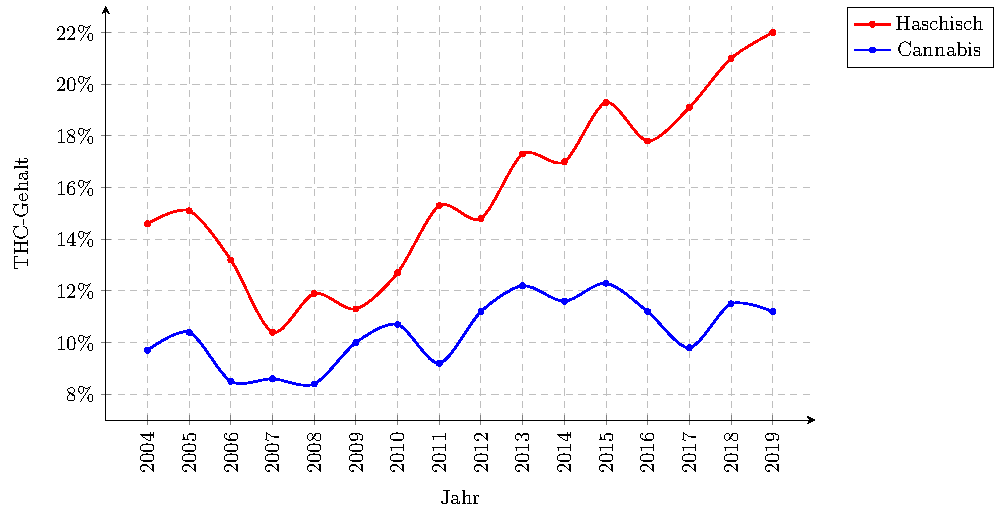
\includegraphics[height=8.5cm]{../figures/thc-statistic}
		\captionsetup{font=small}
		\caption[Entwicklung des THC Gehalts]{Entwicklung des THC Gehalts\protect\footnotemark}		
		\label{fig:thcdevelopment}
	\end{figure}
	\footnotetext{Eigene Abbildung. Vgl. \cite[15-17]{sgrm}.}
	
	
	
\end{document}